\documentclass{article}
\usepackage[
				pdftex,
				colorlinks=true,
				bookmarksnumbered=true,
				bookmarksopen=true,
				bookmarksopenlevel=3,
				pdfstartview=FitP,
				urlcolor=blue,
			]{hyperref}
\pdfinfo{
			/Title(Esercitazione di Laboratorio: Generatori di funzione e filtri RC)
			/Author(Coa Giulio, Licastro Dario, Montano Alessandra)
		}
\usepackage[italian]{babel}
\usepackage{geometry,titling,mdsymbol,stmaryrd,graphicx,subcaption}
\setlength{\columnsep}{1cm}
\graphicspath{{./Image/}}
\renewcommand\maketitlehooka{
								\null
								\mbox{}
								\vfill
							}
\renewcommand\maketitlehookd{
								\vfill
								\null
							}
\title{
		\begin{center}
			Esercitazione di Laboratorio:
		\end{center}
		\newline
		\begin{center}
			Generatori di funzione e filtri RC
		\end{center}
	}
\author{
			Coa Giulio
			\and
			Licastro Dario
			\and
			Montano Alessandra
		}
\begin{document}
	%-----------------------------------------------------------------------------
	%  TITLE
	%-----------------------------------------------------------------------------
	\begin{titlingpage}
		\maketitle
	\end{titlingpage}
	\newpage
	%-----------------------------------------------------------------------------
	%  PURPOSE OF THE EXPERIENCE
	%-----------------------------------------------------------------------------
	\section{Scopo dell'esperienza}
		Lo scopo di questa esercitazione è stato studiare la risposta in frequenza di due filtri RC per mezzo di un segnale sinusoidale di ampiezza e frequenza note.
	%-----------------------------------------------------------------------------
	%  INSTRUMENTATION USED
	%-----------------------------------------------------------------------------
	\section{Strumentazione utilizzata}
		La strumentazione usata durante l'esercitazione è:
		\begin{center}
			\begin{tabular}{ |c|c|c| }
				\hline
				\multirow{\textbf{Strumento}}			   & \textbf{Marca e Modello}	& \textbf{Caratteristiche} \\
				\hline
				\multirow{Multimetro}					   & Agilent 34401A				& \\
				\multirow{Oscilloscopio}				   & Rigol DS1054Z				& 4 canali, \\
														   &							& $ B = 50 \, \mathrm{MHz} $, \\
														   &							& $ f_{\mathrm{c}} = 1 \, \mathrm{G\frac{Sa}{s}} $, \\
														   &							& $ R_{\mathrm{i}} = 1 \, \mathrm{M\Omega} $, \\
														   &							& $ C_{\mathrm{i}} = 13 \, \mathrm{pF} $, \\
														   &							& $ 12 \, \mathrm{Mbps} $ di profondità di memoria \\
				\multirow{Generatore di segnali}		   & Rigol DG1022				& 2 canali, \\
														   &							& $ f_{\mathrm{uscita}} = 20 \, \mathrm{MHz} $, \\
														   &							& $ Z_{\mathrm{uscita}} = 50 \, \mathrm{\Omega} $ \\
				\multirow{Cavi coassiali}				   &							& Capacità dell'ordine dei $ 80 \div 100 \, \mathrm{p\frac{F}{m}} $ \\
				\multirow{Scheda con filtri RC premontati} &							& \\
				\hline
			\end{tabular}
		\end{center}
	%-----------------------------------------------------------------------------
	%  THEORETICAL PREMISES
	%-----------------------------------------------------------------------------
	\section{Premesse teoriche}
		\subsection{Incertezza sulla misura dell'oscilloscopio}
			La misura del valore di un segnale tramite l’oscilloscopio (sia esso l'ampiezza, la frequenza, il periodo, etc.) presenta un'incertezza che dipende, principalmente, da due fattori:
			\begin{itemize}
				\item l’incertezza strumentale introdotta dall’oscilloscopio (ricavabile dal manuale).
				\item l’incertezza di lettura dovuta all’errore del posizionamento dei cursori.
			\end{itemize}
			Quest’ultima incertezza deriva dal fatto che il segnale visualizzato non ha uno spessore nullo sullo schermo.
		\subsection{Filtro RC}
			Un filtro RC è un circuito elettrico del primo ordine composto da una resistenza e da un condensatore.
			\subsubsection{Filtro passa-basso}
				Un filtro passa-basso è un filtro RC che permette il passaggio di frequenze al di sotto di una data soglia, detta frequenza di taglio.
				\begin{figure}[h!]
					\centering
					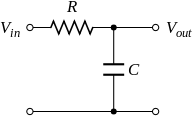
\includegraphics[scale=0.6]{filtroPassaBasso}
					\caption{Circuito corrispondente ad un filtro passa-basso.}
					\label{fig:filtroPassaBasso}
				\end{figure}
				\newline
				\begin{figure}[h!]
					\centering
					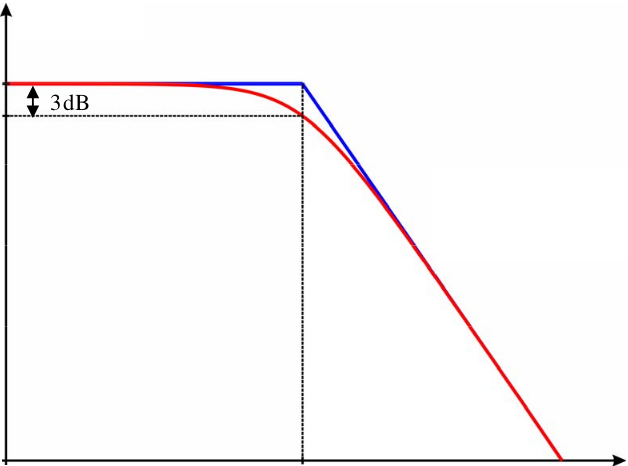
\includegraphics[scale=0.4]{filtroPassaBassoBode}
					\caption{Diagramma di Bode corrispondente ad un filtro passa-basso.}
					\label{fig:filtroPassaBassoBode}
				\end{figure}
			\subsubsection{Filtro passa-alto}
				Un filtro passa-alto è un filtro RC che permette il passaggio di frequenze al di sopra di una data soglia, detta frequenza di taglio.
				\begin{figure}[h!]
					\centering
					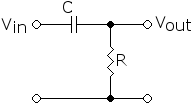
\includegraphics[scale=0.6]{filtroPassaAlto}
					\caption{Circuito corrispondente ad un un filtro passa-alto.}
					\label{fig:filtroPassaAlto}
				\end{figure}
				\newline
				\begin{figure}[h!]
					\centering
					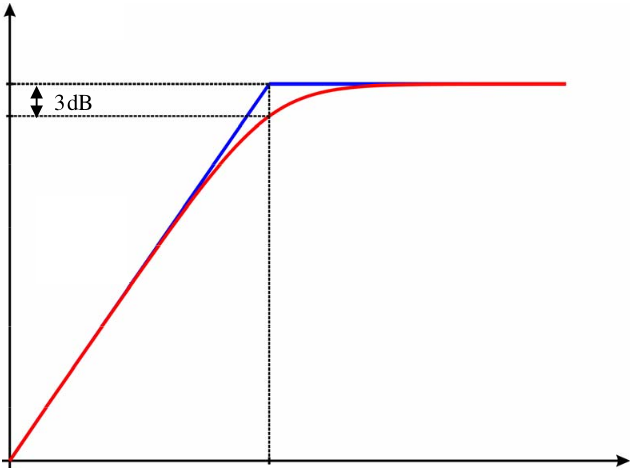
\includegraphics[scale=0.4]{filtroPassaAltoBode}
					\caption{Diagramma di Bode corrispondente ad un filtro passa-basso.}
					\label{fig:filtroPassaAltoBode}
				\end{figure}
				\newpage
			\subsubsection{Filtro passa-banda}
				Un filtro passa-banda è un filtro RC che permette il passaggio di frequenze entro un certo range; questo filtro è caratterizzato dalla presenza di due frequenze di taglio.
				\begin{figure}[h!]
					\centering
					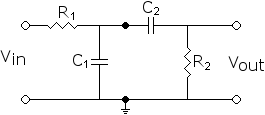
\includegraphics[scale=0.6]{filtroPassaBanda}
					\caption{Circuito corrispondente ad un un filtro passa-banda.}
					\label{fig:filtroPassaBanda}
				\end{figure}
				\newline
				\begin{figure}[h!]
					\centering
					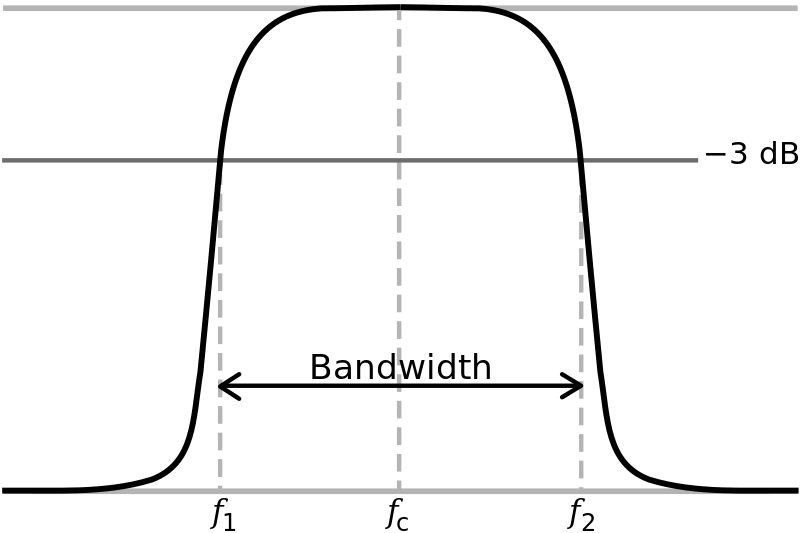
\includegraphics[scale=0.4]{filtroPassaBandaBode}
					\caption{Diagramma di Bode corrispondente ad un filtro passa-banda.}
					\label{fig:filtroPassaBandaBode}
				\end{figure}
	%-----------------------------------------------------------------------------
	%  LABORATORY EXPERIENCE
	%-----------------------------------------------------------------------------
	\section{Esperienza in laboratorio}
		\subsection{Operazioni preliminari}
			Abbiamo regolato il generatore di segnali in modo da visualizzare un segnale sinusoidale di ampiezza $ V_{\mathrm{pp}} = 1 \, \mathrm{V} $ e frequenza $ f = 1 \, \mathrm{kHz} $; successivamente abbiamo collegato il generatore di segnali all'oscilloscopio tramite un cavo coassiale BNC-BNC, di lunghezza pari a $ 1 \, \mathrm{m} $, al fine di visualizzare la forma d'onda, ottentendo il circuito qui rappresentato.
			\begin{figure}[h!]
				\centering
				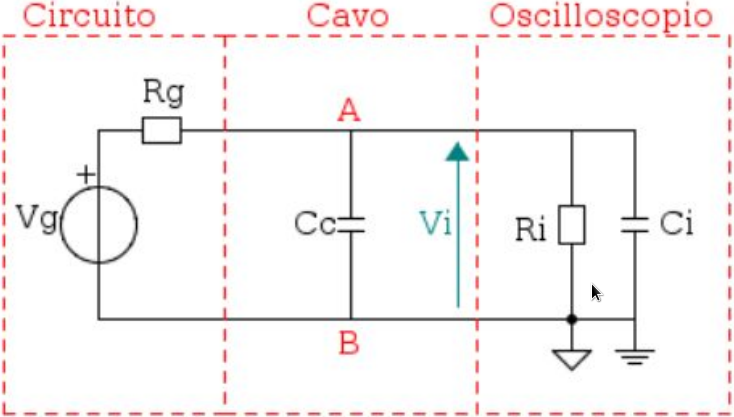
\includegraphics[scale=0.4]{theveninCavoDSO}
				\caption{Generatore di segnali collegato all'oscilloscopio tramite un cavo coassiale BNC-BNC.}
				\label{fig:theveninCavoDSO}
			\end{figure}
		\subsection{Uso dei generatori di segnali}
			\subsubsection{Frequenza dei segnali}
				Dal manuale del generatore di segnali, abbiamo riportato il valore massimo di frequenza che ciascun segnale può raggiungere e, successivamente, abbiamo regolato il generatore in modo da visualizzare un segnale sinusoidale di ampiezza $ V_{\mathrm{pp}} = 1 \, \mathrm{V} $ e frequenza $ f = 1 \, \mathrm{kHz} $, per poi verificarne la frequenza tramite l'uso dell'oscilloscopio e del multimetro.
			\subsubsection{Tipo ed ampiezza dei segnali}
				Dal manuale del generatore di segnali, abbiamo riportato il valore massimo di ampiezza che ciascun segnale può raggiungere e, successivamente, abbiamo regolato il generatore in modo da visualizzare un segnale sinusoidale di ampiezza $ V_{\mathrm{pp}} = 1 \, \mathrm{V} $ e frequenza variabile per misurare i diversi valori picco-picco raggiunti.
				\newline
				Infine, tramite la definizione di $ \mathrm{dB} $, abbiamo ottenuto la frequenza al di sopra della quale il segnale viene attenuato di $ 1 \, \mathrm{dB} $.
			\subsubsection{Offset}
				Abbiamo regolato il generatore di segnali in modo da visualizzare un segnale sinusoidale di ampiezza $ V_{\mathrm{pp}} = 1 \, \mathrm{V} $, frequenza $ f = 1 \, \mathrm{kHz} $ e offset di $ 0.2 \, \mathrm{V} $; a questo punto, abbiamo visualizzato le rappresentazioni in continua (modalità d'accoppiamento in DC) e in alternata (modalità d'accoppiamento in AC) del segnale.
				% IMMAGINI
				\newline
				Infine, abbiamo ripetuto il procedimento per un offset di $ - 0.2 \, \mathrm{V} $.
				% IMMAGINI
		\subsection{Scheda con filtro RC}
			Abbiamo collegato la scheda coi filtri RC premontati al generatore di segnali tramite un cavo BNC-BNC e all'oscilloscopio tramite due cavi coassiali BNC-coccodrillo, uno attaccato a monte della resistenza e uno a valle del dei condensatori.
			\newline
			L'interruttore che gestisce la presenza del secondo condensatore è posto in parallelo al primo condensatore presente nel filtro; quando esso viene chiuso, il secondo condensatore viene collegato in parallelo al circuito, aumentando l'attenuazione del filtro, ovvero la sua frequenza di taglio.
			\begin{figure}[h!]
				\centering
				\begin{subfigure}{0.4\textwidth}
					\centering
					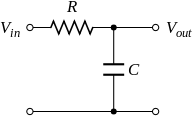
\includegraphics[scale=0.7]{filtroPassaBassoUnCondensatore}
					\caption{Filtro passa-basso con un condensatore.}
				\end{subfigure}
				\begin{subfigure}{0.4\textwidth}
					\centering
					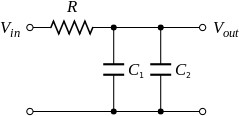
\includegraphics[scale=0.7]{filtroPassaBassoDueCondensatori}
					\caption{Filtro passa-basso con due condensatori.}
				\end{subfigure}
				\label{fig:filtroPassaBassoCondensatori}
			\end{figure}
			\newline
			La resistenza, invece, ha un valore pari a $ 1 \, \mathrm{k\Omega} $; tale valore è stato verificato tramite l'uso del multimetro, ottenendo una misurazione di $ 1'020 \pm 10.2 \, \mathrm{\Omega} $, che rientra nel $ 5 \% $ di tolleranza dato dal costruttore.
		\subsection{Risposta nel dominio della frequenza di un filtro passa-basso: diagrammi di Bode}
			Abbiamo regolato il generatore di segnali in modo da visualizzare un segnale sinusoidale di ampiezza $ V_{\mathrm{pp}} = 800 \, \mathrm{mV} $ e frequenza $ f = 1 \, \mathrm{kHz} $; successivamente abbiamo collegato la scheda coi filtri RC premontati al generatore di segnali tramite un cavo BNC-BNC e all'oscilloscopio tramite due cavi coassiali BNC-coccodrillo, uno attaccato a monte della resistenza e uno a valle del dei condensatori.
			% IMMAGINE
			\newline
			In particolare è stato connesso l'ingresso del filtro al canale $ \mathrm{CH1} $ dell'oscilloscopio, mentre l'uscita è stata connessa al canale $ \mathrm{CH2} $; successivamente, abbiamo impostato il coefficente di deflessione verticale dell'oscilloscopio , per entrambi i canali, a $ 200 \, \mathrm{\frac{mV}{div}} $ e la velocità di scansione orizzontale in modo da poter visualizzare almeno un periodo del segnale.
			\newline
			Infine, abbiamo proceduto col variare la frequenza del segnale al fine di misurare lo sfasamento e l'attenuazione subita da esso, riportando tutti i dati nell'apposita tabella e costruito i relativi grafici.
			Abbiamo ripetuto il procedimento dopo aver chiuso l'interruttore del filtro, inserendo, in parallelo, il secondo condensatore.
		\subsection{Risposta nel dominio della frequenza di un filtro passa-alto: diagrammi di Bode}
			Abbiamo sostituito il filtro passa-basso usato precedentemente con un filtro passa-alto, ovvero abbiamo spostato i cavi coassiali di collegamento sui morsetti del filtro passa-alto presente sulla scheda premontata, ed abbiamo ripetuto l'esperienza.
	%-----------------------------------------------------------------------------
	%  RESULTS
	%-----------------------------------------------------------------------------
	\section{Risultati}
		\subsection{Uso dei generatori di segnali}
			\subsubsection{Frequenza dei segnali}
				I valori massimi di frequenza per i vari segnali del generatore di segnali sono
				\begin{center}
					\begin{tabular}{ |c|c| }
						\hline
						\multirow{\textbf{Tipo di segnale}} & \textbf{Frequenza massima [$ \mathrm{MHz} $]} \\
						\hline
						\multirow{Sinusoidale}				& $ 20 $ \\
						\multirow{Onda quadra}				& $ 5 $ \\
						\multirow{Onda triangolare}			& $ 4 $ \\
						\multirow{Pulsazione}				& $ 5 $ \\
						\hline
					\end{tabular}
				\end{center}
				La frequenza misurata dall'oscilloscopio è pari a
				\newline
				\begin{center}
					$ f = 1 \pm 0.04 \, \mathrm{kHz} $
				\end{center}
				\newline
				Mentre quella misurata dal multimetro è pari a
				\newline
				\begin{center}
					$ f = 999.974 \pm 0.100 \, \mathrm{Hz} $
				\end{center}
			\subsubsection{Tipo ed ampiezza dei segnali}
				I valori massimi di ampiezza per i vari segnali del generatore di segnali sono
				\begin{center}
					\begin{tabular}{ |c|c| }
						\hline
						\multirow{\textbf{Tipo di segnale}} & \textbf{Ampiezza massima [$ \mathrm{V} $]} \\
						\hline
						\multirow{Sinusoidale}				& $ 20 $ \\
						\multirow{Onda quadra}				& $ 20 $ \\
						\multirow{Onda triangolare}			& $ 20 $ \\
						\multirow{Pulsazione}				& $ 20 $ \\
						\hline
					\end{tabular}
				\end{center}
				Mentre i valori dell'ampiezza picco-picco, al variare della frequenza, sono
				\begin{center}
					\begin{tabular}{ |c|c|c|c| }
						\hline
						\multirow{\textbf{Frequenza}}	   & \textbf{Divisioni} & \textbf{Ampiezza divisioni}							& \textbf{Ampiezza cursori [$ \mathrm{mV} $]} \\
						\hline
						\multirow{$ 100 \, \mathrm{Hz} $}  & $ \sim 5 $			& $ 200 \, \mathrm{mV} \cdot 5 = 10.0 \, \mathrm{V} $   & $ 998 $ \\
						\multirow{$ 1 \, \mathrm{kHz} $}   & $ \sim 5 $			& $ 200 \, \mathrm{mV} \cdot 5 = 10.0 \, \mathrm{V} $   & $ 998 $ \\
						\multirow{$ 10 \, \mathrm{kHz} $}  & $ \sim 5 $			& $ 200 \, \mathrm{mV} \cdot 5 = 10.0 \, \mathrm{V} $   & $ 990 $ \\
						\multirow{$ 100 \, \mathrm{kHz} $} & $ \sim 4.8 $		& $ 200 \, \mathrm{mV} \cdot 4.8 = 960 \, \mathrm{mV} $ & $ 963 $ \\
						\multirow{$ 1 \, \mathrm{MHz} $}   & $ \sim 4.8 $		& $ 200 \, \mathrm{mV} \cdot 4.8 = 960 \, \mathrm{mV} $ & $ 950 $ \\
						\multirow{$ 10 \, \mathrm{MHz} $}  & $ \sim 4.4 $		& $ 200 \, \mathrm{mV} \cdot 4.4 = 880 \, \mathrm{mV} $ & $ 890 $ \\
						\hline
					\end{tabular}
				\end{center}
				La tensione per la quale il segnale viene attenuato di $ 1 \, \mathrm{dB} $ è pari a
				\newline
				\begin{center}
					$ 20 \cdot \log_{10} x = -1 \Rightarrow x = 10^{- \frac{1}{20}} = 891 \, \mathrm{mV} $
				\end{center}
				Percui la frequenza sarà di, circa, $ 10 \, \mathrm{MHz} $.
		\subsection{Scheda con filtro RC}
			La frequenza di taglio, con le relative incertezze, dei due filtri passa-basso è
			\newline
			\begin{minipage}[t]{0.5\textwidth}
				\begin{equation*}
					\begin{split}
						f &= \frac{1}{2 \pi \cdot R \cdot C} = \\
						  &= \frac{1}{2 \pi \cdot 1k \cdot X} = \\
						  &= 17 \, \mathrm{kHz}
					\end{split}
				\end{equation*}
				\newline
				\begin{equation*}
					\begin{split}
						\epsilon f &= \epsilon R + \epsilon C = \\
								   &= 0.05 + X = \\
								   &= X
					\end{split}
				\end{equation*}
				\newline
				\begin{equation*}
					\begin{split}
						\delta f &= \epsilon f \cdot f = \\
								 &= X \cdot X = \\
								 &= X \, \mathrm{kHz}
					\end{split}
				\end{equation*}
			\end{minipage}
			\begin{minipage}[t]{0.5\textwidth}
				\begin{equation*}
					\begin{split}
						f &= \frac{1}{2 \pi \cdot R \cdot (C_{1} + C_{2})} = \\
						  &= \frac{1}{2 \pi \cdot 1k \cdot (X + 10n)} = \\
						  &= 8.3 \, \mathrm{kHz}
					\end{split}
				\end{equation*}
				\newline
				\begin{equation*}
					\begin{split}
						\epsilon f &= \epsilon R + \epsilon C_{1} + \epsilon C_{2} = \\
								   &= 0.05 + X + X = \\
								   &= X
					\end{split}
				\end{equation*}
				\newline
				\begin{equation*}
					\begin{split}
						\delta f &= \epsilon f \cdot f = \\
								 &= X \cdot X = \\
								 &= X \, \mathrm{kHz}
					\end{split}
				\end{equation*}
			\end{minipage}
			Mentre quella del filtro passa-alto è
			\begin{equation*}
				\begin{split}
					f &= \frac{1}{2 \pi \cdot R \cdot C} = \\
					  &= \frac{1}{2 \pi \cdot 1k \cdot X} = \\
					  &= 17 \, \mathrm{kHz}
				\end{split}
			\end{equation*}
			\newline
			\begin{equation*}
				\begin{split}
					\epsilon f &= \epsilon R + \epsilon C = \\
							   &= 0.05 + X = \\
							   &= X
				\end{split}
			\end{equation*}
			\newline
			\begin{equation*}
				\begin{split}
					\delta f &= \epsilon f \cdot f = \\
							 &= X \cdot X = \\
							 &= X \, \mathrm{kHz}
				\end{split}
			\end{equation*}
		\subsubsection{Risposta nel dominio della frequenza di un filtro passa-basso: diagrammi di Bode}
			I dati misurati usando il filtro passa-basso con l'interruttore aperto, ovvero sfruttando un solo condensatore, sono
			\begin{center}
				\begin{tabular}{ |c|c|c|c|c| }
					\hline
					\multirow{\textbf{Frequenza}} & \textbf{Tensione in input [$ \mathrm{mV} $]} & \textbf{Tensione in output [$ \mathrm{mV} $]} & \textbf{Fase [\textdegree]} & \textbf{$ H(s) $ [$ \mathrm{dB} $]} \\
					\hline
					\multirow{$ 100 \, \mathrm{Hz} $} & $ 840 \pm 88.0 $ & $ 840 \pm 88.0 $ & $ 1.08 $ & $ 0 $ \\
					\multirow{$ 300 \, \mathrm{Hz} $} & $ 832 \pm 87.6 $ & $ 832 \pm 87.6 $ & $ 1.08 $ & $ 0 $ \\
					\multirow{$ 500 \, \mathrm{Hz} $} & $ 840 \pm 88.0 $ & $ 832 \pm 87.6 $ & $ 1.62 $ & $ -0.0830 $ \\
					\multirow{$ 1 \, \mathrm{kHz} $}  & $ 832 \pm 87.6 $ & $ 832 \pm 87.6 $ & $ 3.50 $ & $ -0.0830 $ \\
					\multirow{$ 3 \, \mathrm{kHz} $}  & $ 832 \pm 87.6 $ & $ 808 \pm 88.4 $ & $ 10.0 $ & $ -0.254 $ \\
					\multirow{$ 5 \, \mathrm{kHz} $}  & $ 832 \pm 87.6 $ & $ 792 \pm 87.6 $ & $ 15.0 $ & $ -0.430 $ \\
					\multirow{$ 10 \, \mathrm{kHz} $} & $ 832 \pm 87.6 $ & $ 704 \pm 87.1 $ & $ 30.0 $ & $ -1.45 $ \\
					\multirow{$ 15 \, \mathrm{kHz} $} & $ 808 \pm 88.4 $ & $ 600 \pm 88.0 $ & $ 41.5 $ & $ -2.58 $ \\
					\multirow{$ 16 \, \mathrm{kHz} $} & $ 808 \pm 88.4 $ & $ 580 \pm 86.7 $ & $ 43.2 $ & $ -3.22 $ \\
					\multirow{$ 18 \, \mathrm{kHz} $} & $ 800 \pm 88.0 $ & $ 552 \pm 87.4 $ & $ 44.0 $ & $ -3.22 $ \\
					\multirow{$ 20 \, \mathrm{kHz} $} & $ 800 \pm 88.0 $ & $ 520 \pm 88.0 $ & $ 50.0 $ & $ -3.64 $ \\
					\multirow{$ 25 \, \mathrm{kHz} $} & $ 800 \pm 88.0 $ & $ 448 \pm 88.7 $ & $ 53.0 $ & $ -5.03 $ \\
					\multirow{$ 30 \, \mathrm{kHz} $} & $ 800 \pm 88.0 $ & $ 392 \pm 87.2 $ & $ 60.0 $ & $ -6.19 $ \\
					\multirow{$ 1 \, \mathrm{MHz} $}  & $ 784 \pm 87.2 $ & $ 22 \pm X $ & $ 92.2 $ & $ -31.0 $ \\
					\hline
				\end{tabular}
			\end{center}
			% IMMAGINI MODULO E FASE
			Mentre i dati misurati usando il filtro passa-basso con l'interruttore chiuso, ovvero sfruttando entrambi i condensatori, sono
			\begin{center}
				\begin{tabular}{ |c|c|c|c|c| }
					\hline
					\multirow{\textbf{Frequenza}} & \textbf{Tensione in input [$ \mathrm{mV} $]} & \textbf{Tensione in output [$ \mathrm{mV} $]} & \textbf{Fase [\textdegree]} & \textbf{$ H(s) $ [$ \mathrm{dB} $]} \\
					\hline
					\multirow{$ 1 \, \mathrm{kHz} $}   & $ 840 \pm 88.0 $ & $ 840 \pm 88.0 $ & $ 6.48 $ & $ 0 $ \\
					\multirow{$ 2 \, \mathrm{kHz} $}   & $ 820 \pm 89.0 $ & $ 780 \pm 87.0 $ & $ 16.6 $ & $ -0.43 $ \\
					\multirow{$ 3 \, \mathrm{kHz} $}   & $ 820 \pm 89.0 $ & $ 760 \pm 88.0 $ & $ 21.1 $ & $ -0.66 $ \\
					\multirow{$ 5 \, \mathrm{kHz} $}   & $ 816 \pm 88.8 $ & $ 688 \pm 88.5 $ & $ 30.6 $ & $ -1.48 $ \\
					\multirow{$ 7 \, \mathrm{kHz} $}   & $ 816 \pm 88.8 $ & $ 620 \pm 89.3 $ & $ 40.0 $ & $ -2.31 $ \\
					\multirow{$ 7.5 \, \mathrm{kHz} $} & $ 808 \pm 88.4 $ & $ 608 \pm 88.5 $ & $ 42.0 $ & $ -2.47 $ \\
					\multirow{$ 8.3 \, \mathrm{kHz} $} & $ 800 \pm 88.0 $ & $ 560 \pm 88.0 $ & $ 43.6 $ & $ -3.10 $ \\
					\multirow{$ 8.5 \, \mathrm{kHz} $} & $ 800 \pm 88.0 $ & $ 560 \pm 88.0 $ & $ 44.0 $ & $ -3.01 $ \\
					\multirow{$ 10 \, \mathrm{kHz} $}  & $ 800 \pm 88.0 $ & $ 512 \pm 87.4 $ & $ 47.9 $ & $ -3.87 $ \\
					\multirow{$ 12 \, \mathrm{kHz} $}  & $ 800 \pm 88.0 $ & $ 460 \pm 86.3 $ & $ 49.1 $ & $ -4.80 $ \\
					\multirow{$ 14 \, \mathrm{kHz} $}  & $ 800 \pm 88.0 $ & $ 440 \pm 88.0 $ & $ 55.3 $ & $ -5.19 $ \\
					\multirow{$ 15 \, \mathrm{kHz} $}  & $ 820 \pm 89.0 $ & $ 420 \pm 90.0 $ & $ 54.1 $ & $ -5.60 $ \\
					\multirow{$ 20 \, \mathrm{kHz} $}  & $ 780 \pm 87.0 $ & $ 320 \pm 88.0 $ & $ 72.1 $ & $ -7.95 $ \\
					\multirow{$ 30 \, \mathrm{kHz} $}  & $ 800 \pm 88.0 $ & $ 260 \pm 85.1 $ & $ 68.9 $ & $ -9.76 $ \\
					\multirow{$ 50 \, \mathrm{kHz} $}  & $ 800 \pm 88.0 $ & $ 180 \pm 84.0 $ & $ 70.4 $ & $ -13.0 $ \\
					\hline
				\end{tabular}
			\end{center}
			% IMMAGINI MODULO E FASE
			\newline
			Nel primo caso, la frequenza per cui si aveva uno sfasamento il più vicino possibile ai $ 45 $ \textdegree è $ 18 \, \mathrm{kHz} $, mentre, nel secondo caso, è $ 8.5 \, \mathrm{kHz} $.
		\subsection{Risposta nel dominio della frequenza di un filtro passa-alto: diagrammi di Bode}
			I dati misurati usando il filtro passa-alto sono
			\begin{center}
				\begin{tabular}{ |c|c|c|c|c| }
					\hline
					\multirow{\textbf{Frequenza}} & \textbf{Tensione in input [$ \mathrm{mV} $]} & \textbf{Tensione in output [$ \mathrm{mV} $]} & \textbf{Fase [\textdegree]} & \textbf{$ H(s) $ [$ \mathrm{dB} $]} \\
					\hline
					\multirow{$ 100 \, \mathrm{Hz} $} & $ 840 \pm 88.0 $ & $ 9 \pm X $ & $ 104 $ & $ -39.4 $ \\
					\multirow{$ 5 \, \mathrm{kHz} $}  & $ 808 \pm 88.4 $ & $ 248 \pm 89.3 $ & $ 74.3 $ & $ -10.3 $ \\
					\multirow{$ 8 \, \mathrm{kHz} $}  & $ 808 \pm 88.4 $ & $ 352 \pm 87.1 $ & $ 67.9 $ & $ -7.22 $ \\
					\multirow{$ 10 \, \mathrm{kHz} $} & $ 808 \pm 88.4 $ & $ 416 \pm 89.6 $ & $ 58.3 $ & $ -5.77 $ \\
					\multirow{$ 15 \, \mathrm{kHz} $} & $ 800 \pm 88.0 $ & $ 536 \pm 89.2 $ & $ 45.3 $ & $ -3.48 $ \\
					\multirow{$ 16 \, \mathrm{kHz} $} & $ 800 \pm 88.0 $ & $ 544 \pm 86.9 $ & $ 48.4 $ & $ -3.35 $ \\
					\multirow{$ 17 \, \mathrm{kHz} $} & $ 800 \pm 88.0 $ & $ 564 \pm 88.3 $ & $ 47.7 $ & $ -3.01 $ \\
					\multirow{$ 18 \, \mathrm{kHz} $} & $ 792 \pm 87.6 $ & $ 580 \pm 86.7 $ & $ 42.1 $ & $ -2.71 $ \\
					\multirow{$ 20 \, \mathrm{kHz} $} & $ 792 \pm 87.6 $ & $ 608 \pm 88.5 $ & $ 41.0 $ & $ -2.30 $ \\
					\multirow{$ 25 \, \mathrm{kHz} $} & $ 792 \pm 87.6 $ & $ 656 \pm 89.0 $ & $ 35.1 $ & $ -1.64 $ \\
					\multirow{$ 29 \, \mathrm{kHz} $} & $ 792 \pm 87.6 $ & $ 680 \pm 88.0 $ & $ 30.6 $ & $ -1.32 $ \\
					\multirow{$ 1 \, \mathrm{MHz} $}  & $ 784 \pm 87.2 $ & $ 776 \pm 88.3 $ & $ 3.60 $ & $ -0.09 $ \\
					\hline
				\end{tabular}
			\end{center}
			% IMMAGINI MODULO E FASE
			\newline
			La frequenza per cui si aveva uno sfasamento il più vicino possibile ai $ 45 $ \textdegree è $ 17 \, \mathrm{kHz} $.
	%-----------------------------------------------------------------------------
	%  CONCLUSION
	%-----------------------------------------------------------------------------
	\section{Conclusioni}
		\subsection{Uso dei generatori di segnali}
			Dai valori riportati si evince la compatibilità fra i valori di frequenza e tensione misurati tramite l'oscilloscopio e quelli impostati nel generatore di segnali; inoltre possiamo notare come il segnale uscente dal generatore tenda ad avere una diminuzione del proprio valore data la non idealità del generatore stesso.
			\subsubsection{Offset}
				In seguito all’aggiunta di un offset al segnale, si nota come quest’ultimo venga traslato verso l’alto, o verso il basso, rispetto all’asse orizzontale; passando dalla modalità DC a quella in AC, è possibile rimuovere tale effetto in quanto, in tale modalità, l’oscilloscopio rimuove la componente continua del segnale, che, nel nostro caso, coincide con il valore di offset.
		\subsection{Risposta nel dominio della frequenza di un filtro passa-basso: diagrammi di Bode}
			Dai valori presenti nelle tabelle e dai relativi diagrammi di Bode, notiamo come, nel filtro passa-basso, la presenza di un secondo condensatore in parallelo al precedente causi un aumento della capacità totale ed un conseguente abbassamento della frequenza di taglio del circuito.
\end{document}